\section{MMU: Memory Management Unit}

\subsection{Introducción}
En cualquier kernel el manejo de memoria es una parte fundamental. Nuestro kernel no es la excepción. El kernel cuenta con dos niveles de administración
de memoria. De estos dos niveles, la \textit{Unidad de Administración de Memoria}, o \textit{MMU} por sus siglas en inglés (Memory Management Unit) se encarga de administrar la memoria física. 
Es decir, de manejar correctamente y lo mejor posible las páginas y todo lo que concierne al respecto. \\
El modelo de memoria elegido para nuestro kernel hace uso de paginación, aunque no asi de la unidad de Segmentación (sólo lo mínimo necesario para ser funcional). La mmu se encarga entonces 
de administrar las páginas físicas. La forma de administración es relativamente sencilla para el nivel de complejidad del kernel. Los marcos de páginas libres se mantienen en una pila, 
pudiendo extraer del mismo y asociarlos a direcciones virtuales. También se permite liberarlos devolviéndolos a la pila. A continuación se explica más detalladamente cómo se administra la memoria 
y las funciones y mecanismos para ello.

\subsection{Estructuras de la MMU}
La memoria física se divide en unidades de tamaño 4kb llamadas frames o marcos de página. Cada vez que la mmu otorga un sector de memoria a una tarea u otro módulo del kernel que lo requiera, lo 
hace en estas unidades básicas. La tarea principal de la MMU será entonces mantener de alguna forma coherente, la cantidad de frames que aún quedan libres, cuales son, y cuales están siendo ocupados.

\begin{figure}[H]
\centering
\subfloat{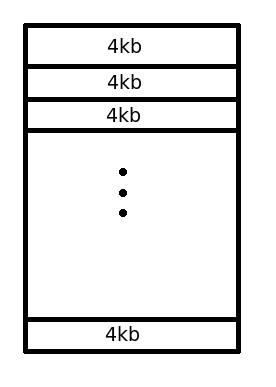
\includegraphics[width=0.4\textwidth]{imagenes/mmu_page_frames.png}}
\caption{Memoria física dividida en sectores contiguos de tamaño 4kb}
\end{figure}

Cada frame de la memoria física se representa con la siguiente estructura

\begin{verbatimtab}
typedef struct page_frame
{
   struct page_frame* next; //proximo frame de la lista de frames libres
   struct page_frame* prev; //frame anterior de la lista de frames libres
   uint32_t ref_count;  //cantidad de referencias externas
} page_frame_t;
\end{verbatimtab}

La mmu mantiene un array llamado \textit{mem\_page\_frames} de estructuras \textit{page\_frame\_t}, una por cada frame físico. A su vez existe una pila de frames libres apuntada por 
\textit{free\_page\_frame\_stack}. Los punteros \textit{next} y \textit{prev} sirven entonces para formar una lista doblemente enlazada entre los frames que esten libres. Un frame esta libre 
si y sólo si su cantidad de referencias es nula. Es decir, no existe ninguna virtual address de ninguna tarea ni proceso que haga referencia al frame. De esta forma se obtiene una estructura 
como la que se muestra a continuación:

\begin{figure}[H]
\centering
\subfloat{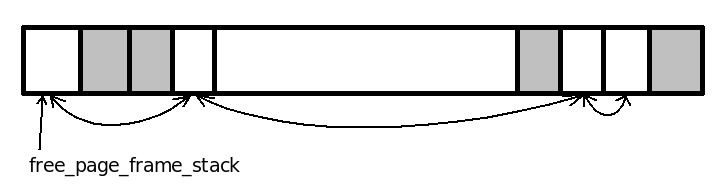
\includegraphics[width=0.8\textwidth]{imagenes/mmu_page_frames_array.png}}
\caption{Memoria física dividida en sectores contiguos de tamaño 4kb}
\end{figure}

\subsection{Inicialización de la MMU}
Para poder construir la estructura anteriormente descripta, es necesario que el kernel conozca la cantidad de memoria con la que cuenta. La mmu cuenta con una función que se encarga de inicializar 
todo lo necesario, incluyendo un conteo de la cantidad de memoria total. Este trabajo es llevado a cabo por la función \textit{mmu\_init}. El prototipo de la función es 

\begin{verbatimtab}
 /**
 * Inicializa la Memory Management Unit. Para ello utilizando la informacion provista 
 * por GRUB inicializa las estructuras de control de memoria y se encarga de llamar 
 * a las funciones necesarias para instalar la GDT definitiva y pasar a paginacion
 *
 * @param mdb Puntero a estructura multiboot_info_t provista por GRUB al inicio del kernel
 * @see mmu_install_gdt
 * @see mmu_init_paging
 * @see mmu_build_kernel_heap
 */
void mmu_init(multiboot_info_t* mbd);
\end{verbatimtab}

La estructura \textit{multiboot\_info\_t} es una estructura provista por GRUB al momento de booteo. Esta estructura provee, entre otros datos, un mapa de la memoria física, describiendo 
no sólo la cantidad de memoria disponible, sino también qué sectores están reservados por otros dispositivos como el BIOS y cuales están libres para uso del SO. Utilizando esto, la mmu 
inicializa el array de frames, marcando como ocupados aquellos que corresponden a sectores reservados. Un esquema simplificado de los pasos que realiza \textit{mmu\_init} sería

\begin{verbatimtab}
 mmu_init
      Contar la memoria disponible
      Correr el puntero __kernel_end tanto como ocupe mem_page_frames

      Para cada frame
	  Si la direccion del frame corresponde a un sector reservado
	  o a una direccion del kernel, marcarlo como ocupado
	  Si no, como libre.

      Inicializar paginacion

      Instalar GDT definitiva
\end{verbatimtab}

\subsection{Paginación y la MMU}
Como ya dijimos, nuestro kernel utiliza el modelo de paginacón. El mapeo realizado por el kernel es bastante sencillo. Las direcciones del kernel comienzan a partir de 0x80000000, mientras que 
el espacio de usuario esta reservado entre los 0 y 2 primeros GB. Para que el kernel utilice estas direcciones, es linkeado por un linker script especial. Sin embargo, el bootloader carga 
el kernel en las primeras direcciones. Para poder ejecutar el código sin problemas, se instala una GDT provisoria, cuyos segmentos son especialmente definidos para que cuando la unidad de segmentación 
traduce las direcciones, la dirección resultante sea \textit{d} + 0x80000000. De esta forma el código puede ejecutar sin problemas.\\
Dentro de \textit{mmu\_init} dijimos que se inicializan las estructuras de paginación. La PDT del kernel es apuntada por \textit{kernel\_pdt} (definida en mmu.c). La PDT se construye entonces 
mapeando el kernel desde los 2GB en adelante, utilizando páginas de 4mb para que las traducciones de la TLB se realice en forma más eficientemente ya que el procesador utiliza una TLB distinta.
Asi mismo, también se mapea el kernel a partir de la dirección 0x0 con un propósito: en el momento de transición entre activar paginación e instalar la GDT definitiva (recordando que teníamos una provisoria) 
todo siga funcionando. Cuando iniciamos paginación, comienza a actuar una unidad de traducción adicional de direcciones. Dado que sigue en acción la GDT provisoria, ahora las direcciones que antes 
eran físicas, pasan por la traducción de la PDT. Al haber mapeado el kernel a partir de 0x0 todo funciona correctamente. Finalmente instalamos una GDT definitiva utlizando segmentos de 4gb, por lo que 
las direcciones lineales ahora son traducidas por el mapeo desde los 2gb en adelante.

\subsection{Interfaz de la MMU}
Para que la MMU pueda ser utilizada, se define en mmu.h su interfaz pública. Las funciones que expone son las siguientes

\subsubsection{mmu\_alloc}
\begin{verbatimtab}
uint8_t mmu_alloc(uint32_t *pdt, uint32_t *va, uint32_t *pa, uint8_t perm);
\end{verbatimtab}
Toma un frame fisico libre de 4kb y lo mapea dentro de la primera direccion virtual disponible para la 
PDT pasada como parametro con los permisos solicitados. Devuelve ademas la direccion fisica asociada.\\
Parámetros:
\begin{itemize}
 \item \textbf{pd} Puntero a la pdt sobre la cual se quiere realizar el mapeo.
 \item \textbf{va} Puntero donde se guarda la direccion virtual donde se realizo el mapeo
 \item \textbf{pa} Puntero donde se guarda la direccion fisica
 \item \textbf{perm} Permisos asignados a la pagina mapeada
\end{itemize}


\subsubsection{mmu\_alloc\_at\_VA}
\begin{verbatimtab}
 uint8_t mmu_alloc_at_VA( pde_t *pdt, uint32_t va, uint8_t perm, uint8_t force_dealloc );
\end{verbatimtab}
Obtiene un frame libre y lo intenta mapear en la direccion virtual pasada como parametro.\\
Parámetros:
\begin{itemize}
 \item \textbf{pdt} Puntero a la PDT sobre la cual se realiza el mapeo
 \item \textbf{va} Direccion virtual usada para mapear el frame libre
 \item \textbf{perm} Permisos asignados a la nueva pagina mapeada
 \item \textbf{force\_dealloc} Si en la va pasada como parametro ya habia un mapeo previo, entonces lo deshace si force\_dealloc==1
\end{itemize}
Devuelve E\_MMU\_SUCCESS si se realizo el mapeo correctamente, E\_MMU\_INVALID\_VA si ya habia un mapeo y force\_dealloc==0 o E\_MMU\_NO\_MEMORY si no se pudo realizar.

\subsubsection{mmu\_map\_pa2va}
\begin{verbatimtab}
 uint8_t mmu_map_pa2va(pde_t *pdt, uint32_t pa, uint32_t va, uint8_t perm, uint8_t force_dealloc );
\end{verbatimtab}
Intenta asociar la va con la pa pasada como parametro para la pdt solicitada.\\
Parámetros:
\begin{itemize}
 \item \textbf{pdt} Puntero a la PDT sobre la cual se realiza el mapeo
 \item \textbf{va} Direccion fisica usada para realizar el mapeo
 \item \textbf{va} Direccion virtual usada para mapear la direccion fisica
 \item \textbf{perm} Permisos asignados a la nueva pagina mapeada
 \item \textbf{force\_dealloc} Si en la va pasada como parametro ya habia un mapeo previo, entonces lo deshace si force\_dealloc==1
\end{itemize}
Devuelve E\_MMU\_SUCCESS si se realizo el mapeo correctamente, E\_MMU\_INVALID\_VA si ya habia un mapeo y force\_dealloc==0 o E\_MMU\_NO\_MEMORY si no se pudo realizar

\subsubsection{mmu\_free}
\begin{verbatimtab}
 uint8_t mmu_free( pde_t *pdt, uint32_t va );
\end{verbatimtab}
Dada una PDT, deshace el mapeo de la va, obtiene el frame correspondiente, decrementa su cantidad de 
referencias (si son 0 lo apila como libre) y realiza invlpg para limpiar la TLB. \\
Parámetros:
\begin{itemize}
  \item \textbf{pdt} Puntero a una PDT.
  \item \textbf{va}  Direccion virtual a liberar. Debe ser multiplo de PAGE\_SIZE
\end{itemize}
Devuelve E\_MMU\_SUCCESS si la operacion se realizo con exito, o E\_MMU\_INVALID\_VA si la va no pudo ser desmapeada.

\subsubsection{mmu\_get\_free\_frame\_count}
Devuelve la cantidad de frames libres en memoria fisica
\begin{verbatimtab}
 mmu_get_free_frame_count(); 
\end{verbatimtab}

\subsubsection{mmu\_install\_task\_pdt}
\begin{verbatimtab}
 uint8_t mmu_install_task_pdt(uint32_t *va, uint32_t *pa);
\end{verbatimtab}
Instala una nueva PDT para ser usada por una nueva tarea.\\
Parámetros:
\begin{itemize}
 \item \textbf{va} Es un puntero a un uint32\_t que se va a utilizar para guardar la va utilizada para mapear la nueva pdt dentro del contexto del kernel.
 \item \textbf{pa} Es un puntero a un uint32\_t que se va a utililar para guardar la pa utilizada para guardar la nueva pdt.
\end{itemize}
Devuelve E\_MMU\_SUCCESS si se realizó con exito la instalación, o E\_MMU\_NO\_MEMORY si no hubo memoria disponible para realizar la operación.

\subsubsection{mmu\_kalloc}
\begin{verbatimtab}
 uint8_t mmu_kalloc( uint32_t *va );
\end{verbatimtab}
Toma un frame fisico libre de 4kb y devuelve su dirección virtual en el contexto del kernel.\\
Parámetros:
\begin{itemize}
  \item \textbf{va}  Puntero donde se guarda la dirección virtual.
\end{itemize}
Devuelve E\_MMU\_SUCCESS si se pudo realizar el alloc correctamente, o E\_MMU\_NO\_MEMORY en caso de error.


\subsection{Funciones internas de la MMU}
A continuación enumeramos las funciones definidas en mmu.c que no son parte de la interfaz pública

\subsubsection{mmu\_init\_paging}
\begin{verbatimtab}
static void mmu_init_paging(uint32_t *kpdt);
\end{verbatimtab}
Inicializa la PDT del kernel, mapeando la memoria fisica en forma lineal a partir 
de KERNEL\_VIRTUAL\_START utilizando paginas de KERNEL\_PAGE\_SIZE (4mb). \\
Parámetros:
\begin{itemize}
 \item \textbf{kpdt} Puntero a la page directory table del kernel
\end{itemize}

\subsubsection{mmu\_install\_gdt}
\begin{verbatimtab}
static void mmu_install_gdt();
\end{verbatimtab}
Instala la GDT definitiva, quitando la dummy gdt utilizada durante el proceso de booteo.

\subsubsection{mmu\_push\_free\_frame}
\begin{verbatimtab}
static void mmu_push_free_frame(page_frame_t* page_frame);
\end{verbatimtab}
Toma un puntero a un frame y lo almacena en la pila de frames libres. Solo se debe hacer push de frames con cantidad de referencias igual a 0. \\
Parámetros:
\begin{itemize}
 \item \textbf{page\_frame} Puntero al page\_frame\_t a liberar
\end{itemize}

\subsubsection{mmu\_pop\_free\_frame}
\begin{verbatimtab}
static page_frame_t* mmu_pop_free_frame();
\end{verbatimtab}
Saca un frame del stack de frames libres y devuelve un puntero a este. \\
Devuelve un puntero del tipo\textit{ page\_frame\_t*}. Si no hay frames libres, devuelve NULL.

\subsubsection{mmu\_page\_frame\_2\_PA}
\begin{verbatimtab}
static uint32_t mmu_page_frame_2_PA(page_frame_t* page_frame);
\end{verbatimtab}
Devuelve la direccion fisica del frame pasado como parametro. Para ello se fija en el puntero al frame, y lo compara con el puntero 
al principio de la lista para conocer su posicion y luego multiplicar convenientemente para conocer la direccion fisica del mismo.\\
Parámetros:
 \begin{itemize}
  \item \textbf{page\_frame} Puntero al page\_frame cuya physical address se quiere conocer
 \end{itemize}

\subsubsection{mmu\_PA\_2\_page\_frame}
\begin{verbatimtab}
static page_frame_t* mmu_PA_2_page_frame(uint32_t physical_address);
\end{verbatimtab}
Toma una direccion fisica y devuelve un puntero page\_frame\_t al frame correspondiente en el array 
mem\_page\_frames. No quita el frame de la lista de libres.\\
Parámetros:
\begin{itemize}
 \item \textbf{physical\_address} Direccion fisica del frame. Debe ser multiplo de PAGE\_SIZE.
\end{itemize}
Devuelve un puntero page\_frame\_t* al frame asociado, o NULL si la direccion fisica es inválida.

\subsubsection{ mmu\_get\_page\_frame}
\begin{verbatimtab}
static page_frame_t* mmu_get_page_frame(uint32_t physical_address);
\end{verbatimtab}
Dada una direccion fisica, devuelve el frame asociado a esta, pero lo quita de la lista de libres (si es que lo estaba) incrementando la cantidad de referencias.\\
Parámetros:
\begin{itemize}
 \item \textbf{physical\_address} Direccion fisica del frame. Debe ser multiplo de PAGE\_SIZE.
\end{itemize}
Devuelve un puntero page\_frame\_t* al frame asociado, o NULL si la direccion fisica es inválida.


\subsubsection{mmu\_free\_page\_frame}
\begin{itemize}
 \item \textbf{frame} Puntero al frame a liberar
\end{itemize}
Decrementa las referencias del frame pasado como parametro. Si llegan a ser nulas, se agrega a la pila de libres.


\subsubsection{mmu\_alloc\_page}
\begin{verbatimtab}
 static uint8_t mmu_alloc_page(pde_t *pdt, page_frame_t *page_frame, uint32_t va, uint8_t perm, uint8_t force_dealloc);
\end{verbatimtab}
Asocia la direccion virtual va con el frame apuntado por page\_frame para la PDT pasada como parametro, utilizando los permisos perm. 
Si la va ya estaba siendo utilizada para otro mapeo, force\_dealloc indica si se deshace el mapeo anterior o no.\\
Parámetros:
 \begin{itemize}
  \item \textbf{pdt} Puntero a la PDT sobre la cual se va a realizar el mapeo.
  \item \textbf{page\_frame} Puntero a un marco de pagina.
  \item \textbf{va} Virtual address a utilizar para el mapeo.
  \item \textbf{perm} Permisos con los que se va a mapear la pagina.
  \item \textbf{force\_dealloc} Si vale 1, fuerza el desmapeo de cualquier mapeo anterior.
 \end{itemize}
Devuelve E\_MMU\_SUCCESS si todo salio correctamente. E\_MMU\_INVALID\_VA si la va ya estaba mapeada y force\_dealloc==0. E\_MMU\_NO\_MEMORY si no hubo memoria.

\subsubsection{mmu\_dirwalk}
\begin{verbatimtab}
 static uint8_t mmu_dirwalk(pde_t *pdt, uint32_t va, pte_t **pte, uint8_t create_page_table, uint8_t ptable_domain);
\end{verbatimtab}
Recorre las tablas y hace apuntar pte a la page table entry que corresponde de acuerdo a la va pasada como parametro y la PDT. \\
Parámetros:
\begin{itemize}
  \item \textbf{pdt} Puntero a la PDT sobre la cual se va a realizar el mapeo.
  \item \textbf{va} Virtual address a utilizar para el mapeo.
  \item \textbf{pte} Puntero doble a una pte\_t. Dentro de pte se guarda la pte correspondiente a la va para la PDT.
  \item \textbf{create\_page\_table} Si la va no tiene una page table creada, create\_page\_table==1 hace que se cree dicha tabla, de lo contrario no se crea y mmu\_dirwalk devuelve error
\end{itemize}
Devuelve E\_MMU\_SUCCESS si todo salio correctamente. E\_MMU\_PTABLE\_NOT\_PRESENT si la tabla de paginas para la va no existe y create\_page\_table==0. 
 E\_MMU\_NO\_MEMORY si no hubo memoria suficiente para realizar la operacion. 

\subsubsection{mmu\_get\_pte}
\begin{verbatimtab}
 static pte_t* mmu_get_pte(pde_t *ptd, uint32_t va);
\end{verbatimtab}
Devuelve un puntero a la la pte asociada a la va pasada como parámetro.\\
\begin{itemize}
  \item \textbf{pdt} Puntero a la PDT sobre la cual se va a realizar el mapeo.
  \item \textbf{va} Virtual address a utilizar para el mapeo.
\end{itemize}
Devuelve un puntero a la pte asociada o NULL si no existe la page table.
